\subsection{Vue d'ensemble et système de coordonnées}\label{chapter-LHC-section-CMS-subsec-overview_and_coordinates}

\begin{figure}[h]
\centering
\includegraphics[width=\textwidth]{\PhDthesisdir/plots_and_images/CMS_slices/from_CMS_document_13631-v4/cms_160312_06-FR.tex}
\caption[Vue éclatée du détecteur CMS.]{Vue éclatée du détecteur CMS~\cite{CMS_document_13631-v4}.}
\label{fig-chapter-LHC-section-CMS-subsec-overview_and_coordinates-vue_eclatee_CMS}
\end{figure}

\begin{figure}[h]
\centering
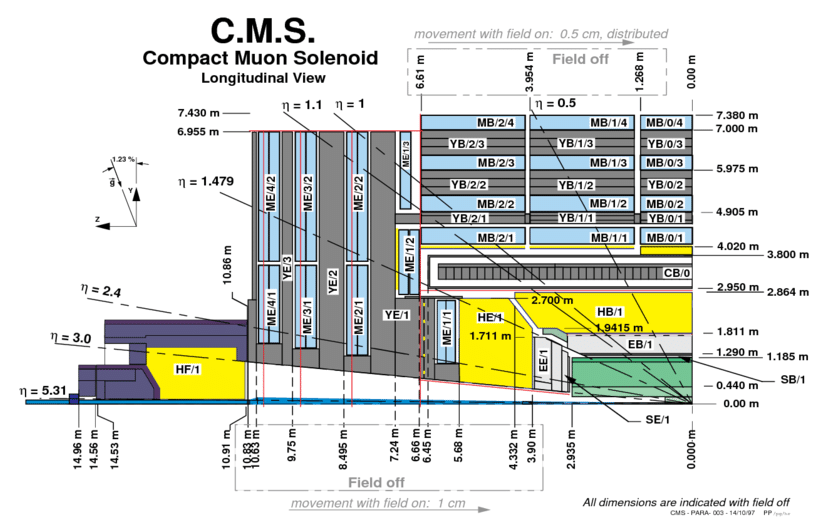
\includegraphics[width=\textwidth]{\PhDthesisdir/plots_and_images/from_CMS_alignment_photodetectors/CMS-eta-ranges.png}
\caption[Vue longitudinale d'un quadrant du détecteur CMS.]{Vue longitudinale d'un quadrant du détecteur CMS~\cite{CMS_alignment_photodetectors}. Les directions correspondant à quelques valeurs de pseudo-rapidité sont illustrées et des mesures de distances par rapport au centre du détecteur, lieu des collisions, sont indiquées. Le sol de la caverne présente une inclinaison de \SI{1.23}{\%} par rapport à la direction de la gravité locale $\vec{g}$, ce que montre le schéma à gauche.}
\label{fig-chapter-LHC-section-CMS-subsec-overview_and_coordinates-CMS-eta-ranges}
\end{figure}